\documentclass[a4paper,10pt]{article}

%====================== PACKAGES ======================

\usepackage[utf8]{inputenc}
\usepackage[french]{babel}
\usepackage{graphicx}
\usepackage{hyperref}
\usepackage{array}
\usepackage{tabularx}
\usepackage{setspace}
\usepackage[T1]{fontenc}
\usepackage[top=2.5cm, bottom=2.5cm, left=2cm, right=2cm]{geometry}
\usepackage{fancyhdr}
\usepackage{wrapfig}
\usepackage{filecontents}
\usepackage{tikzsymbols}
\usepackage{metre}

%====================== INFORMATION ET REGLES ======================


\hypersetup{
pdfauthor = {Julien Schoumacher},
pdftitle = {Stage de fin d'étude -
           Etude de sécurité d'un contrôleur SDN : ONOS},
pdfsubject = {Mémoire de stage d'ingénieur},
pdfkeywords = {SDN, ONOS, sécurité},
pdfstartview = {FitH}}

\graphicspath{ {images/} }


%====================== Bibliographie ======================
\begin{filecontents}{references.bib}
@online{of_def,
  title = {Avantages SDN},
  url = {https://www.opennetworking.org/sdn-resources/sdn-definition},
}

@online{indirection,
  title = {Niveau d'indirection supplémentaire},
  url = {https://en.wikipedia.org/wiki/Fundamental_theorem_of_software_engineering},
}

@online{rapport_maxence,
  title = {Mémoire de stage : Étude d’OpenFlow dans le contexte de la sécurité},
  author = {Maxence Tury}
}

@online{histoire,
  title = {A Survey of Software-De ned Networking:  Past,
Present, and Future of Programmable Networks},
  author = {Bruno Nunes Astuto, Marc Mendonça, Xuan Nam Nguyen, Katia Obraczka,Thierry Turletti}
  url = {https://hal.inria.fr/hal-00825087/file/hal_final.pdf}
}

@online{openflow_google,
  title = {Openflow at Google},
  author = {Hoelzle Tue}
  url = {http://opennetsummit.org/archives/apr12/hoelzle-tue-openflow.pdf}
}

@online{OF_10,
  title = {Spécification Openflow 1.0},
  url = {http://archive.openflow.org/documents/openflow-spec-v1.0.0.pdf}
}

@online{OF_15,
  title = {Spécification Openflow 1.5},
  url = {https://www.opennetworking.org/images/stories/downloads/sdn-resources/onf-specifications/openflow/openflow-switch-v1.5.0.noipr.pdf}
}

@online{OF_13,
  title = {Spécification Openflow 1.3},
  url = {https://www.opennetworking.org/images/stories/downloads/sdn-resources/onf-specifications/openflow/openflow-spec-v1.3.0.pdf}
}
\end{filecontents}


%======================== DEBUT DU DOCUMENT ========================
\newgeometry{top=3.5cm}
\pagestyle{fancy}
\fancyhf{}
\fancyhead[C]{~\\}
\fancyfoot[C]{\thepage}

\begin{document}



%page de garde
\begin{titlepage}
	\newcolumntype{s}{>{\hsize=.25\hsize}X}
	\begin{tabularx}{\textwidth}{lsrl}
		
\includegraphics[width=0.2\textwidth]{TelecomParisTech_logo_200_01.png}
		&
    	\shortstack{\huge{Télécom} \\ \huge{ParisTech}}
    	&
		
\includegraphics[width=0.2\textwidth]{Logo_SP.jpg}
		&
		\shortstack{\huge{Télécom} \\ \huge{SudParis}}
	\end{tabularx}

    \begin{center}
        \vspace*{1cm}
        
        \Huge
       	~\\
       	~\\
       	~\\
        \textbf{Mémoire de stage}
        
        \vspace{0.5cm}
        \LARGE
        Sécurité d'un contrôleur SDN : ONOS\\
        ~\\
        
        \vspace{1.5cm}
        
        \textbf{Julien Schoumacher}
        
        \vfill
       
        \begin{flushleft}
       		 Diplôme préparé : Ingénieur\\
        	 Stage effectué du 20 juillet 2016 au 20 janvier 2017 à Télécom SudParis sous la direction de Grégory Blanc
        \end{flushleft}
        \vspace{0.3cm}
        
    \end{center}
\end{titlepage}

%======================== Remerciements ========================
\newpage
~
\section*{\Huge{Remerciements\\}}
\Large Avant d'entamer la lecture de ce rapport, je tiens avant tout à remercier toute l'équipe du département RST (Réseaux et Services des Télécommunications) de Télécom SudParis qui m'a si bien accueilli durant ce stage. Je remercie également mon encadrant côté Télécom ParisTech Rida Khatoun, m'ayant mis en relation avec le maître de conférences Gregory Blanc qui m'a encadré avec bienveillance pendant toute la durée du stage. Enfin, toutes les autres personnes que j'ai pu cottoyer plus ou moins longtemps à l'occasion d'évènements ponctuels comme la conférence RAID qui s'est tenue en septembre.
\phantomsection


%======================== Table des matières ========================
\newpage
\tableofcontents


\newpage
\fancyhead[L]{1- Réseau SDN}
\section{Réseau SDN (Software Defined Network)}
	\subsection{Motivation}
		On ne peut pas entamer cette étude portant en partie sur les réseaux SDN sans oublier de mentionner quelques éléments difficilement contestables sur les réseaux actuels \footnote{\label{of_def}Aussi résumé dans \url{https://www.opennetworking.org/sdn-resources/sdn-definition}} :

\begin{itemize}

\item La demande ne cesse de croître : on observe un accroissement considérable des enjeux liés au traitement de masse importante de données, de l'utilisation de services cloud, du trafic mobile et peut être bientôt de l'utilisation d'objets connectés. Or tous ces éléments présentent le point commun de communiquer avec de nombreuses entités situées sur des réseaux potentiellement éloignés. Cela mobilise donc un trafic réseau intense.

\item Les technologies actuelles pour soutenir cette demande énorme sont capables de fournir un débit titanesque : que l'on considère des technologies sans fil ou non, au coeur des réseaux tant au niveau des terminaux des utilisateurs, on atteint aujourd'hui des débits théoriques de l'ordre du Gigabit par seconde pour l'utilisateur. Tout cela sans que l'on ait vraiment conscience des conditions que cela requiert.

\item Les méthodes d'accès sont aujourd'hui bien différentes. Précédemment le modèle client/ serveur était largement employé, avec dans le cas d'une entreprise, un réseau interne constitué de plusieurs LAN séparés, et connecté à internet de manière quasiment unique. Cela entraînant une configuration possiblement statique et donc aisée, les échanges se déroulant principalement sur un mode requête/réponse. Or la tendance, notamment à cause des deux premiers points, est à l'émergence de nouveaux modes d'accès plus horizontaux (avec d'avantage d'entités faisant circuler l'information au même niveau "hiérarchique"). Ce type de communication tient entre autres de la distribution plus éparse des données à travers le réseau due au grossissement de la taille des bases de données, à la duplication de celles-ci (mise en cache sur différents serveur à travers le monde pour permettre un accès plus rapide), à l'augmentation du trafic volumineux (vidéo, voix) et de nouveaux trafics (IoT, Bring Your Own Device, ...) même au sein de l'entreprise. Enfin, l'utilisation de plus en plus répandue de services cloud, avec ses implications au niveau de la virtualisation (que ce soit des applications, ou bien des bases de données), susceptible de changer en permanence la localisation des serveurs pour garantir une certaine flexibilité.

\end{itemize}

Or, le réseau principal global tel que nous le connaissons (la partie reposant sur TCP/IP en tout cas) a été conçu d'abord dans un but de fiabilité : chaque paquet doit être reçu, peu importe la route empruntée. L'architecture distribuée actuelle n'est donc pas bâtie pour assurer spécifiquement une extension aisée des services fournis, ni une qualité de service définie. Le routeur (et le réseau d'ailleurs) des années 1980 a donc été progressivement amélioré sur la base de ce paradigme initial, avec le plan de données et le plan de contrôle attachés aux mêmes équipements, configurés en partie manuellement. Tout s'est complexifié également : nouveaux protocoles, ajouts d'équipements spécifiques (capables de répartir la charge réseau, de filtrer les paquets, de prévenir de certaines tentatives d'attaque, etc ...), ...\\
Certains éléments de réflexion peuvent éventuellement nous mettre sur la voie d'une complexité qui, à défaut d'être exponentielle, l'est d'avantage que simplement linéaire (c'est du moins une conviction personnelle non vérifiée) :

\begin{itemize}
\item Plus il y a d'éléments statiques dans un réseau, et plus la propagation des modifications d'ensemble est coûteuse (puisqu'il faut penser à chaque impact sur les parties statiques et modifier un à un chaque équipement).
\item Si un problème survient, il est difficile d'avoir une vue globale de ce qui se passe puisqu'à moins de disposer d'équipements spéciaux aucune vue globale du réseau n'est accessible : il faut vérifier (potentiellement) que chaque élément se comporte correctement et est bien configuré.
\item Les interfaces entre switchs, routeurs et autres éléments peuvent varier selon le constructeur, et le logiciel sur les équipements est souvent propriétaire et complexe, surtout dans le cas de gros réseaux hétérogènes, ce qui ne facilite pas forcément la bonne marche de l'ensemble.
\end{itemize}

De nombreux problèmes se résolvent avec un niveau d'abstraction supplémentaire \footnote{\label{indirection}\url{https://en.wikipedia.org/wiki/Fundamental_theorem_of_software_engineering}}. Si le dévelop-pement de systèmes de plus en plus complexes s'est fait de manière très rapide sur PC, c'est d'abord grâce à la première couche d'abstraction qu'ont constitué les instructions assembleur, puis à la seconde qu'a été le système d'exploitation. Certaines personnes ont eu l'idée, au lieu de considérer le réseau comme un élément périphérique, de le voir comme un processeur capable d'exécuter des instructions basiques, fournissant de fait un service plus facilement adaptable. C'est sur ce principe que repose le Software Defined Network (SDN). Avec une couche d'abstraction supplémentaire que constitue le protocole choisi pour véhiculer le flot d'instructions (OpenFlow dans notre cas, mais il y en a d'autres que nous évoquerons succintement plus tard), et un système d'exploitation spécifique (Network Operating System, NOS), l'idée est de découpler les différents chemins qu'empruntent les données et le plan de contrôle, à la manière d'un système d'exploitation qui sépare le code d'un programme et les données qu'il utilise.
		~\\
	\subsection{Concepts}
		La dernière analogie (avec un ordinateur) peut être poursuivie de la manière suivante. Sur un PC classique, on crée et utilise des applications qui reposent sur un système d'exploitation responsable des éléments matériels. De manière similaire, le modèle SDN permet la création d'applications "réseau" sans se soucier de la traduction des décisions de routage des paquets au niveau applicatif en routage au niveau des interfaces physiques.\\

Pour réaliser cela, il est nécessaire, puisqu'un réseau est constitué d'entités physiquement séparées, de disposer d'un protocole de communication standard entre celles-ci. Mais ça n'est pas suffisant : des instructions de routage doivent également être distribuées. Cela n'est possible que si il existe un cerveau central qui coordonne les opérations (il n'existe pas vraiment d'intelligence collective à ce jour). C'est le rôle du contrôleur SDN. On déporte ainsi l'intelligence humaine déployée dans la configuration de tous les éléments du réseau vers un seul (même si il peut être dupliqué).\\

\begin{figure}[h]
  	\centering
  	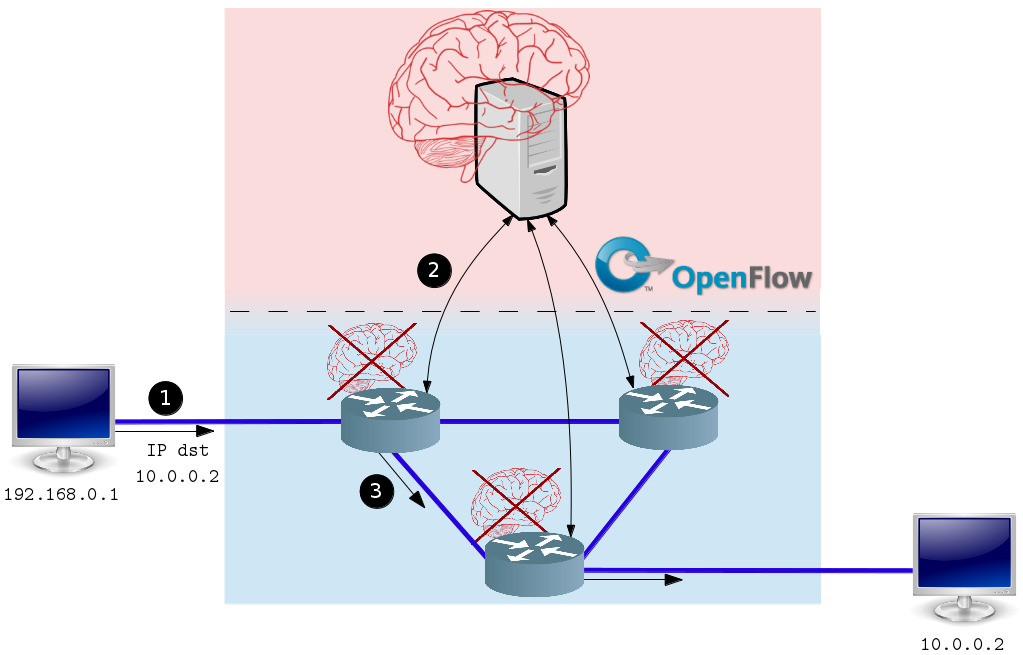
\includegraphics[width=0.8\textwidth]{openflow.png}
  	\caption[Caption for LOF]{Réseau SDN : "l'intelligence" est déportée vers le contôleur \footnotemark}
\end{figure}

\footnotetext{\label{rapport_maxence} Schéma extrait du mémoire "Étude d’OpenFlow dans le contexte de la sécurité" de Maxence Tury}

\begin{figure}[h]
  	\centering
  	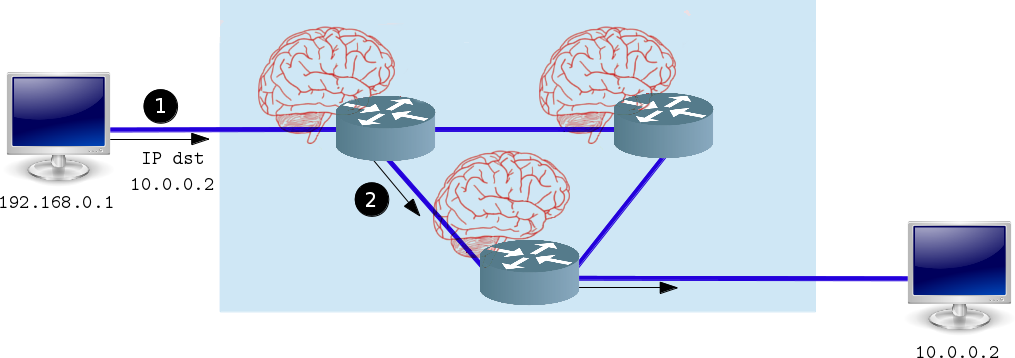
\includegraphics[width=0.85\textwidth]{routage_normal.png}
  	\caption{Réseau classique : chaque routeur contient une partie de la logique de contrôle}
\end{figure}

Les avantages de cette architecture sont multiples :
\begin{itemize}
\item D'abord cela réduit grandement la complexité de configuration manuelle et le risque d'erreur (si le système d'exploitation réseau est fiable).
\item Cela facilite donc énormément le développement d'applications réseau complexes, puisque la tâche peut être quasiment séparée de sa réalisation physique.
\item Les routes optimales sont plus facilement calculables qu'au sein d'un réseau classique : un seul élément gère les différentes distances et métriques qui peuvent changer selon le trafic, et être modifiées à la volée par des applications spécifiques.
\item La gestion du réseau devient plus simple, les évènements importants (perte d'un lien, dysfonctionnement, ralentissement ...) peuvent être remarqués rapidement, la réaction pouvant être automatique et quasiment instantanée.
\item Les coûts matériels sont globalement diminués puisqu'un switch programmable Openflow peut n'implémenter que le protocole en question pour être fonctionnel (le reste pouvant être pris en charge logiciellement au niveau du contrôleur). Il est également possible de migrer partiellement vers une architecture SDN en utilisant des switchs hybrides.
\end{itemize}

Pour résumer, beaucoup plus de flexibilité est permise par cette approche, économisant temps et matériel. Évidemment, l'idée n'est pas nouvelle, mais n'a pas que des avantages. Notamment : la sécurité du contrôleur devient un point brûlant, puisque toute la gestion du réseau repose sur lui.
		~\\
	\subsection{Historique}
		L'idée d'une séparation entre plan de données et plan de contrôle n'est pas nouvelle, et cette partie se propose de retracer succinctement diverses voies qui ont abouti à l'adoption assez univoque du protocole OpenFlow comme interface entre les deux. Pour obtenir un état de l'art détaillé et complet, il est possible de consulter les articles "A Survey of Software-Defined Networking: Past, Present, and Future of Programmable Networks"\footnote{\label{histoire}\url{https://hal.inria.fr/hal-00825087/file/hal_final.pdf}} (2014) et "Software-Defined Networking: A Comprehensive Survey"\footnote{\url{http://www.hit.bme.hu/~jakab/edu/litr/SDN/Long_Survey_06994333.pdf}} (2015).\\

Assez tôt est apparue l'idée de rendre les switchs programmables : dès 1990, le groupe Open Signaling propose un protocole de contrôle de switchs à distance appelé GSMP (General Switch
Management  Protocol). Si les possibilités restent assez limitées (essentiellement gestion des ports, redirection de trafic sur des ports contrôlés, et obtention de statistiques), cela permet néanmoins un accès au matériel plus aisé.

D'autres approches sont testées dans la même période : l'initiative Active Networking propose quant à elle un mécanisme de propagation de code que l'équipement réseau exécute lorsqu'il reçoit les paquets encapsulant le code (même si cela pose un gros problème en matière de sécurité).

Le groupe DCAN (Devolved Control of ATM Networks) propose une approche qui se rapproche très fortement du paradigme SDN : ils développent un protocole minimaliste entre une entité spécialisée (le contrôleur) et autres équipements et mettent en place une gestion semi-automatique du réseau pour partitionner les ressources disponibles (ils rajoutent donc la possibilité de programmer le contrôleur).\\

Le projet 4D \footnote{\url{http://www.cs.cmu.edu/~4D/}} initié en 2004, présente une formalisation du concept : on cherche à obtenir la possibilité de prendre des décisions réseau en dehors des équipements physiques, ce qui nécessite l'obtention d'un maximum d'informations à la fois sur la composition physique du réseau, et sur les liens qui existent entre chaque élément. L'incorporation des services globaux que sont la découverte de la topologie et la dissémination d'informations sur l'état général du réseau associée à la possibilité d'agir sur le réseau est ce qui a inspiré l'idée de système d'exploitation réseau, qu'implémentent aujourd'hui les contrôleurs SDN.\\

On peut encore citer NETCONF et Ethane (2006), le premier pouvant être vu comme une extension de SNMP, le second comme un ancêtre immédiat d'OpenFlow. Même si la finalité d'Ethane était plus axée sur une gestion des identités (vérification des droits d'un paquet à circuler sur le réseau entre autres) que sur une gestion générale du réseau, c'est un protocole entre switch programmable et contrôleur encapsulant des actions à effectuer sur des paquets reçus au niveau du switch (ces actions étant essentiellement limitées à de la redirection/suppression).\\

OpenFlow a quant à lui précédé l'apparition du terme SDN lors d'expérimentations à Stanford vers 2010 (la première spécification d'OpenFlow pour la production (1.0.0), a été publiée début 2010).
		~\\
	\subsection{Exemples d'applications}
		En 2011, l'Open Networking Foundation (ONF) est créée. Regroupant des gros acteurs comme Google, Yahoo, Facebook, Verizon, Microsoft ou encore Deutsche Telekom, c'est l'organisme principal qui encourage l'adoption de la technologie SDN, en publiant régulièrement de nouvelles spécifications Openflow.\\

Google, en 2012, présente, pour la première fois, une architecture SDN pour ses datacenters, utilisant Openflow sur des switchs conçus par eux-mêmes (étant pionniers, leur position étant qu'ils auraient utilisé des switchs existants si ceux-ci implémentaient toutes les fonctionnalités Openflow leur étant nécessaires). Grâce à ce nouveau paradigme, Google affirme (en 2012) obtenir des performances dix fois supérieures en terme de débit, et surtout utiliser 100\%\footnote{\url{http://www.networkworld.com/article/2189197/lan-wan/google-s-software-defined-openflow-backbone-drives-wan-links-to-100--utilization.html}} de leurs lignes (contrairement aux 30 à 40\% en vigueur dans l'industrie, notamment pour garantir un service même en cas de nombreuses pannes, ce qui n'est plus nécessaire avec un réseau SDN qui adapte automatiquement le routage pour pallier aux problèmes).\\

Microsoft semble également s'être intéressé au SDN pour son service "Azure" depuis quelques années maintenant \footnote{\url{http://www.networkworld.com/article/2937396/cloud-computing/microsoft-needs-sdn-for-azure-cloud.html}}, et de manière générale toutes les figures de proue de l'industrie  numérique (celles qui disposent de nombreux serveurs et gèrent des flux énormes et grandissants de données comme Amazon, AT\&T, Facebook, ...) se sont plus ou moins annoncées investies dans le processus, possiblement avec leur propre protocole SDN. Si des grosses entreprises ont annoncé l'utilisation de ce type de réseau, les données précises concernant les performances obtenues sont difficilement accessibles, ce qui rend compliquée l'évaluation des avantages réels de SDN.\\

Par ailleurs, les switchs compatibles Openflow, ou les switchs Openflow seuls, que fournissent (depuis 2011 environ) certaines entreprises majeures du domaine comme Brocade, HP, IBM, Juniper ou encore NEC, Pronto ou Pica8, manquent encore parfois de maturité (RFC parfois interprétée différemment, vulnérabilités spécifiques, ...). L'évolution des versions Openflow est également parfois difficile à suivre (la spécification de la version 1.0.0 (fin 2009) fait 42 pages\footnote{\label{OF_10}\url{http://archive.openflow.org/documents/openflow-spec-v1.0.0.pdf}}, celle de la dernière version stable (1.5.0, fin 2014) en fait 277 \footnote{\label{OF_15}\url{https://www.opennetworking.org/images/stories/downloads/sdn-resources/onf-specifications/openflow/openflow-switch-v1.5.0.noipr.pdf}}). Or l'industrie dans ce domaine présente une certaine inertie (peu sont les compagnie qui proposent des switchs compatibles avec la dernière version d'Openflow, certaines vendant encore des switchs Openflow 1.0).\\

Les applications semblent donc d'un premier abord limitées aux datacenters (beaucoup de données à traiter, grande variabilité de la topologie (les machines virtuelles changent souvent d'emplacement/adresse)). En réalité, SDN peut être utilisé de manière effective dans plusieurs cas :

\begin{list}{$\Asteriscus$}{}
\item Réseaux d'entreprises/universités : dans le cas de nombreux équipements/protocoles différents utilisés, SDN permet théoriquement de faciliter le déploiement de politiques réseau complexes.
\item Réseaux optiques : faciliter la transition, la gestion et l'incorporation des réseaux optiques au sein du réseau actuel.
\item Infrastructure based WAN (réservé aux entreprises disposant de nombreux serveurs à travers le monde) : à la manière de Google, un moyen de connecter de grosses entités en évitant les goulots d'étranglement. Egalement un moyen envisageable pour un utilisateur de se connecter depuis n'importe quel endroit en disposant des services auxquels il souscrit.
\item Infrastructure personnelle, petites entreprises : surveiller le trafic et alerter l'administrateur local ou le fournisseur internet en cas de détection d'activité réseau suspecte (utile notamment dans le cadre de l'IoT).\\
\end{list}

Au final, une technologie pouvant sembler prometteuse, mais demeurant assez peu utilisée pour plusieurs raisons. Nous allons en étudier deux d'entre elles par la suite : la sécurité générale du réseau, et l'importance capitale du contrôleur qui devient quasiment l'unique clé de voûte du système.
\newpage
\fancyhead[L]{2- Cadre de l'étude}
\section{Cadre de l'étude}
	\subsection{Problématique et objectifs}
		Mon stage, dont le sujet n'était pas complètement fixé au départ, a pris la tournure suivante : d'abord une étude des réseaux SDN (ne connaissant pas le domaine), puis début d'expérimentations sur le protocole Openflow, avec Scapy et Wireshark. Ensuite, constitution d'un rapide état de l'art en matière d'attaques (générales) sur les réseaux SDN. Puis, l'orientation s'est faite sur l'étude plus précise d'un contrôleur SDN particulier (ONOS), avec la conception de scénarios d'attaque, suivie de leur réalisation.\\
Comme on l'a dit au-dessus, le contrôleur SDN est le point névralgique de toute l'infrastructure. Si on le compromet d'une manière où d'une autre, les conséquences peuvent être désastreuses. L'étude a donc eu pour but de déterminer les principaux vecteurs d'attaque envisageables dans ce genre de réseau, principalement concernant le contrôleur ONOS (principalement, parce qu'il  est possible d'appliquer une majorité des attaques sur d'autres contrôleurs, même si cela n'a pas été expérimentalement vérifié).\\
Pour résumer, un audit (se voulant le plus exhaustif possible, même si il est impossible de couvrir l'ensemble des vulnérabilités d'un tel élément logiciel) a été réalisé. Cet audit a été conçu informellement à partir de la méthode STRIDE\footnote{STRIDE = Spoofing, Tampering, Repudiation, Info disclosure, Denial of service, privilege Escalation, qui respectivement permettent de vérifier les propriétés d'authentification, d'intégrité, de non-répudiation, de confidentialité, de disponibilité et d'autorisation} (utilisée par microsoft à la base, cette manière de modéliser les menaces dans le domaine de la sécurité s’est beaucoup répandue). Certains scénarios ont été expérimentés pour prouver la faisabilité d'attaques précises (donc sous certaines hypothèses qui sont décrites). D'autres faiblesses sont également détaillées dans leur aspect théorique sur la base de sources externes. Bien que n'ayant pas eu accès à une situation réelle de déploiement SDN, j'essaierai de donner une conclusion pas trop biaisée aux tests effectués, et formulerai quelques recommandations et remarques.
	\subsection{Architecture d'un réseau SDN}
		Avant toute chose, il est nécessaire de détailler la façon dont un réseau SDN fonctionne, afin que les attaques qui seront évoquées plus tard puissent être bien comprises. Pour cela, on insistera particulièrement sur la description du protocole Openflow, mais aussi sur celle de l'objet de notre étude, ONOS.
		\subsubsection{Openflow}
			Openflow est un des protocoles qui permet de séparer le plan de données et le plan de contrôle (protocole majoritairement utilisé à l'heure actuelle, étant non propriétaire et porté par l'ONF). Pour l'utiliser, il est nécessaire de disposer de switchs compatibles, c'est à dire des switchs capables de gérer des paquets Openflow. Ainsi, les décisions prises au niveau du contrôleur sont transmises aux switchs concernés par le biais de ce protocole. Pour que l'abstraction de la gestion du réseau soit intéressante, le protocole permet aux switchs une gestion assez fine des paquets reçus à leur niveau, et ce jusqu'au niveau 4 (pour TCP comme on va le voir après). C'est le principal élément de ce qu'on appelle l'interface sud d'un réseau SDN (interface entre contrôleur et entités matérielles) :
\begin{figure}[h]
  	\centering
  	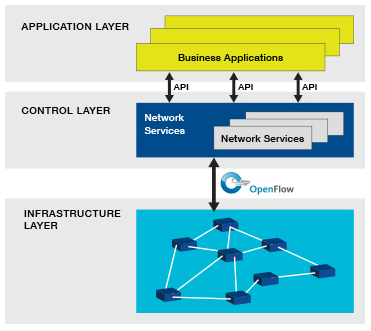
\includegraphics[width=0.45\textwidth]{interfaces.jpg}
  	\caption{Différentes interfaces, Openflow = interface sud}
\end{figure}

Chaque switch (qu'il soit compatible Openflow ou virtuel) consiste en plusieurs tables de flux et une table de groupe (non présente en version 1.0), ainsi qu'un (ou plusieurs) canal(aux) vers le(s) contrôleur(s) (sécurisé(s) via TLS obligatoire en version 1.0 mais obligation supprimée dès la version 1.1 pour des raisons de facilité de déploiement). La description du fonctionnement qui suit est celle de la version 1.3 du protocole (ça n'est donc ni la dernière version, ni la première, mais celle que j'ai principalement utilisée durant le stage, Wireshark la disséquant complètement).\\

La notion de flux est essentielle. Un flux est constitué de 3 parties :
\begin{list}{$\Asteriscus$}{}

\item La première une règle qui filtre les paquets : en fonction des attributs du paquet à l'entrée du switch (port d'entrée physique, adresse ethernet source, adresse ethernet destination, type de paquet, VLAN id, VLAN priority, adresse IP source, adresse IP destination, protocole IP, ToS IP, TCP port source, TCP port destination entre autres). Il est possible de générer des filtrages généraux avec l'utilisation de jokers (wildcard en anglais) sur les champs souhaités (par exemple, si on veut autoriser toutes les adresses ethernet source ayant pour adresse IP x.x.x.x, on pourra utiliser un joker sur le champ adresse ethernet source).

\item La seconde est un compteur qui permet de tenir à jour, si le switch le permet, des statistiques sur l'utilisation du flux.

\item La troisième est une action à appliquer en cas de correspondance du paquet : si le paquet remplit les conditions du filtre, plusieurs types de traitements sont possibles. Entre autres : envoyer le paquet au contrôleur, rediriger le paquet vers un port physique spécifique, vers une table de flux, vers tous les ports sauf le port d'entrée, vers les switchs voisins mis à jour par spanning tree, supprimer le paquet, ou encore modifier certains champs avant redirection, rediriger le paquet vers une queue. Bref, toutes les opérations envisageables sur un paquet. Certaines de ces actions doivent être prises en charge par les switchs Openflow pour que ceux-ci puissent être considérés comme tels. D'autres actions sont optionnelles (par exemple la redirection vers les switchs mis à jour par spanning tree).

\end{list}

Chaque nouveau flux ajouté au switch par le contrôleur l'est dans une table de flux spécifiée. Ainsi, plutôt que d'avoir à organiser relativement la priorité de chaque flux, des regroupements peuvent se faire par table pour factoriser certains traitements. Le switch parcourt chaque table de flux (en considérant le premier flux de chaque table) jusqu'à trouver un filtrage correct pour le paquet. A ce moment, le paquet parcourt et subit les traitements de chacun des flux dans la table trouvée (c'est la notion de pipeline Openflow) jusqu'à ce qu'une action de redirection soit trouvée. La redirection peut également être faite vers une table de flux de priorité inférieure (pour éviter qu'un paquet boucle indéfiniment).

\begin{figure}[h]
  	\centering
  	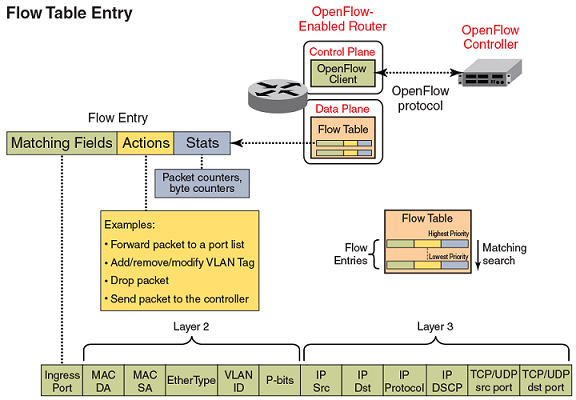
\includegraphics[width=0.9\textwidth]{brocade_flow.png}
  	\caption{Flux et table de flux}
\end{figure}

Basiquement, on peut résumer le protocole Openflow comme étant le protocole permettant :
\begin{list}{$\Asteriscus$}{}

\item de mettre à jour ces tables de flux : ajouts, ajouts partiels (par exemple ajouts de précisions à un flux avec joker), suppressions, modifications, etc ....  

\item d'obtenir des statistiques sur certains éléments (en Openflow 1.3, on peut accéder aux statistiques des flux, des tables, des ports, des queues, des groupes, ou encore du débit (pour la qualité de service)).

\item d'obtenir des informations sur les entités du réseau (nom de l'équipement, nom du fabricant, débit supporté ...)

\end{list}

C'est un protocole qui s'établit de manière classique sur une session TCP (éventuellement surmonté d'une session TLS), habituellement sur les ports 6633 ou 6653 (ce dernier étant maintenant alloué pour cet usage par l'IANA).\\
Il est constitué :

\begin{list}{$\Asteriscus$}{}

\item de messages symétriques (Hello, Echo), qui s'utilisent pour ou démarrer une session Openflow ou s'assurer que les deux parties sont encore connectées

\item de messages contrôleur vers switch (ressemblant à du requête/réponse), généralement les messages qui permettent au contrôleur d'obtenir des informations sur le switchs et de lui donner des ordres. Mais aussi, et c'est important, un message qui permet directement d'insérer du trafic dans le réseau. Ainsi, lorsque le switch envoie un paquet qu'il ne sait pas traiter au contrôleur, celui-ci peut le renvoyer au switch (après l'avoir traité et éventuellement modifié), ce qui évite de perdre le paquet \footnote{On appelle alors ce paquet OFPT\_PACKET\_OUT (selon la spécifiation) qu'on abrégera par la suite en PACKET\_OUT}.

\item de messages asynchrones émis par les switchs, qui sont par exemple susceptibles d'informer le contrôleur lorsqu'ils ont modifié, supprimé ou ajouté un flux, mais également lorsqu'un paquet ne correspond à aucun flux, qu'une erreur survient ou bien qu'un port physique change de configuration. Le message asynchrone le plus important est sûrement celui qui survient lorsque le switch doit envoyer le paquet au contrôleur \footnote{Paquet appelé OFPT\_PACKET\_IN (selon la spécifiation) qu'on abrégera par la suite en PACKET\_IN} (soit parce qu'une règle le demande explicitement, soit parce que le switch ne peut pas traiter le paquet et que la règle par défaut associée demande un envoi au contrôleur).

\end{list}

Ci-dessus une capture Openflow réalisée sous Wireshark.

La figure précédente provient de mes expérimentations, j'ai en effet été amené durant mon stage à créer une sorte de mini-switch virtuel très basique avec Scapy, ce qui m'a forcé à implémenter à la fois la pile TCP et la session Openflow . Même si par la suite cela m'a été peu utile pour réaliser mes scénarios d'attaque, cela m'a permis de bien comprendre le protocole Openflow.

Le lecteur désirant rentrer dans les détails techniques peut se référer à la spécification de la version 1.3\footnote{\label{OF_13}https://www.opennetworking.org/images/stories/downloads/sdn-resources/onf-specifications/openflow/openflow-spec-v1.3.0.pdf (106 pages, dont 49 d'explications)}.
		\subsubsection{Contrôleur SDN}
			Le contrôleur est, comme on l'a déjà dit précédemment, l'élément central du réseau SDN, puisqu'il offre au niveau de son interface nord, une API pour développer des applications réseau, et, au niveau de son interface sud, il contrôle les entités réseaux se chargeant du plan de données, avec le protocole Openflow.

Pour fonctionner correctement, le contrôleur doit avoir la représentation interne la plus exacte possible de la topologie réseau qu'il dirige. Pour cela, Openflow prévoit certains paquets spécialisés. Mais ce n'est pas suffisant, puisque les switchs eux-mêmes ne sont pas capables de renseigner le contrôleur sur la topologie alentours. C'est pourquoi certains mécanismes sont mis en place (qui dépendent généralement du contrôleur, même si, devant utiliser des protocoles classiques compréhensibles par des switchs, les possibilités restent limitées).\\
Le mécanisme que j'ai été amené à constater est celui de l'utilisation de paquets LLDP fabriqués par le contrôleur et envoyés aux switchs sous forme de PACKET\_OUT. En recevant un tel paquet, un switch va le retransmettre en broadcast aux switchs alentours, qui, normalement, sont configurés pour le renvoyer en PACKET\_IN au contrôleur (comportement par défaut, si aucun flux gérant ce type de paquet n'est spécifié, ce qui est préférable). Or, un PACKET\_IN encapsule toutes les informations nécessaires au contrôleur pour mettre à jour la topologie locale : en vérifiant que c'est bien lui qui est à l'origine de l'émission du paquet LLDP initial (avec un champ spécial par exemple), il sait que le switch émetteur du PACKET_IN est relié au switch auquel il avait précédemment envoyé un PACKET_OUT, ces premiers étant des encapsulations de paquets réels circulant sur le réseau, on peut donc y lire des adresses ethernet, des adresses IP, .... La question de la confiance relative à la réception de tels paquets est cruciale et on va voir par la suite qu'il est relativement aisé d'attaquer le contrôleur par ce biais.

//image de l'échange LLDP

Au sein du contrôleur même, on trouve tout le logiciel nécessaire pour lier les informations reçues depuis les différentes entités du réseau aux intentions de plus haut niveau émises. Comme sur un système d'exploitation classique, on peut trouver une abstraction plus ou moins riche : 
		\subsubsection{ONOS}
			ONOS\footnote{Open Network Operating System} est un contrôleur SDN open source récent (début en décembre 2014, la fondation Linux arrive en octobre 2015 dans le projet), écrit en java, déployable avec Maven et utilisant apache-karaf comme conteneur OSGi (qui fournit entre autre l’interface utilisateur permettant l’interaction avec le contrôleur).
La version actuelle est Goldeneye (juin 2016) (1.6), la prochaine Hummingbird.
C'est un projet basé sur la technique \footnote{\url{http://onosproject.org/governance/}} : \begin{quote}
goal is to « provide an environment that thrives on technical meritocracy. Merit is based on technical contribution, not on financial contribution. »
\end{quote}

Le contrôleur est architecturé de la manière suivante :
\begin{figure}[h]
  	\centering
  	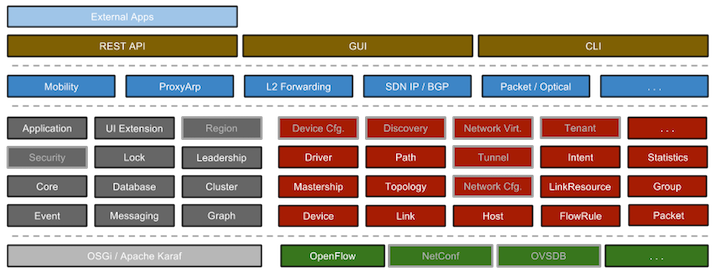
\includegraphics[width=1\textwidth]{ONOS_archi.png}
  	\caption{Architecture logicielle d'ONOS (schéma extrait du site officiel)}
\end{figure}

\begin{list}{$\Asteriscus$}{}

\item Au Sud : une API (southbound) gérant plusieurs protocoles (dont Openflow (toutes les versions jusqu’à la version 1.5, la version 1.6 étant en cours de prise en charge)). C’est la partie d’ONOS qui se charge de la communication avec les switchs. Il est ainsi possible de prendre en charge de nouveaux protocoles ou de nouveaux drivers.

\item Sur le côté : un protocole d’échange entre contrôleurs. Cela permet un contrôle partagé du réseau. Pour cela, des informations sur la topologie de celui-ci doivent être échangées entre contrôleurs. Le protocole en question n'est pas standardisé.

\item Au Nord : une API (northbound) permettant d’écrire des applications utilisant les ressources offertes par le contrôleur. Si le secure mode est activé (nous reviendrons plus en détail sur cela ultérieurement), l’ensemble des méthodes utilisables est restreint. 

\item Au Nord encore : une interface utilisateur fournie par Karaf et composée de 3 parties: une API REST accessible sur le port 8181 (configurable), une interface web (permettant de visualiser l’état du réseau, les applications lancées ...) accessible sur ce même port, et une CLI accessible en SSH sur le port 8101 (ou bien directement sur le contrôleur, là encore tout est configurable).

\end{list}
	\subsection{Surface d'attaque}
		Pour tester le contrôleur, l’installation suivante est actuellement réalisée :
- une machine virtuelle utilisant l'émulateur réseau mininet, qui crée des switchs et hôtes virtuels, et qui permet de générer du trafic réseau SDN.
- une machine virtuelle (ubuntu server) sur laquelle le contrôleur ONOS est installé et est accessible.
- une machine virtuelle (ubuntu desktop) permettant d’intéragir avec le contrôleur en SSH (on peut aussi utiliser la machine non virtuelle).

On va donc appliquer la méthode STRIDE aux divers éléments et interfaces qui composent ONOS, à la manière de ce qui est présenté dans un article de l'institut Fraunhofer \footnote{\url{http://publica.fraunhofer.de/eprints/urn_nbn_de_0011-n-4046948.pdf}}.

		\subsubsection{Menaces au niveau de l'interaction avec les switchs}
			Le contrôleur reçoit et interprète des données des switchs qu'il contrôle. Cela signifie que, si l'une des entités avec qui il communique est malveillante, celle-ci a la possibilité d'agir négativement sur le contrôleur.
En appliquant la méthode STRIDE à l'interface sud, on trouve 4 menaces :

\begin{itemize}

\item Usurpation d'identité (S) : possibilité pour un élement de se faire passer pour ce qu’il n’est pas (un switch se faisant passer pour un autre switch par exemple, ...).

\item Altération (T) : possibilité de modifier le flux de données des switchs en se plaçant sur le chemin du contrôleur (man in the middle). Cette partie est rapide à étudier puisque TLS, si il est correctement utilisé, permet d’éviter toute modification du flux.

\item Divulgation d'information (I) : possibilité d’obtenir les flux d’informations entre les éléments du réseau et le contrôleur (là encore si TLS est activé cela réduit la menace à son minimum).

\item Déni de service (D) : possibilité de surcharge des interfaces réseau, par exemple un switch non désiré sur le réseau qui surcharge le contrôleur de messages, de manière intelligente (en sachant ce qui ralentira le plus le contrôleur) ou non.

\end{itemize}

Dans la suite, on testera S, T, D (et pas I car on supposera TLS activé). Mais toujours relativement au contrôleur, c'est à dire qu'on regardera si le contrôleur agit comme il est supposé réagir, permettant ou non l'attaque. Et on constatera ou non la généricité des attaques.

		\subsubsection{Menaces au niveau de l'interaction utilisateur}
			Le contrôleur exécute potentiellement des applications fournies par des tiers. Si un utilisateur  importe une application malveillante sur le contrôleur, cela peut avoir des répercussions sur tout le réseau.
Concernant la méthode STRIDE appliquée à l'interface nord, on trouve majoritairement 5 menaces :

\begin{list}{$\Asteriscus$}{}

\item Spoofing (S) : (abus de langage ici, mais c'est la catégorie qui se rapproche le plus de la réalité) possibilité de modifier le comportement de certaines applications avec des droits non adaptés.

\item Tampering (T) : possibilité de modifier le flux de données des applications en se plaçant sur le chemin du contrôleur (man in the middle). Cette partie est rapide à étudier puisque là encore, TLS, si il est correctement utilisé, permet d’éviter toute modification du flux d'information.

\item Repudiation (R) : possibilité pour une application de nier certaines actions dont elle est l'origine.

\item Information disclosure (I) : possibilité d’obtenir des informations sur d'autres applications, sur l'état général du contrôleur, ...

\item Denial of service (D) : possibilité d'action néfaste sur le contrôleur (modification de la topologie, dégradation du débit offert par le contrôleur, ...).

\end{list}

Dans la suite, on testera S,T,D et I. Encore une fois cela sera fait par rapport à ONOS, ce qui ici se justifie d'avantage (aucun standard n'existant au niveau de l'interface nord, celle-ci peut varier beaucoup selon le contrôleur). De plus, ONOS propose un mécanisme de sécurité intéressant à étudier qui est le Security Mode, mis en place depuis la version Drake (1.3) du contrôleur.

\begin{figure}[h]
  	\centering
  	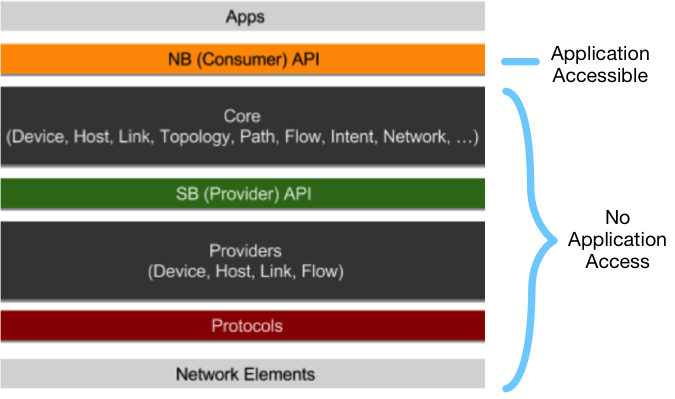
\includegraphics[width=0.6\textwidth]{secure_mode.png}
  	\caption{Secure mode activé : accès aux fonctions critiques restreint lors de l'utilisation de l'API par certaines applications}
\end{figure}

Ce module, qui continue d'être amélioré, rajoute la possibilité de définir des permissions fines (ce qui se traduit par le droit d'utiliser ou non certaines fonctions de l'API) par rôle aux applications, et sera légèrement détaillé plus tard. Les attaques qui constitueront cette partie seront donc moins génériques que les attaques menées au niveau de l'interface sud.

		\subsubsection{Autres menaces}
			Nous avons évoqué les menaces qui pesaient sur les interfaces nord et sud, mais il existe encore d'autres menaces :

\begin{itemize}

\item Sur le contrôleur en lui même : bien que cela soit laborieux et que je n'aie pas réussi à le faire durant mon stage, il n'est pas impossible qu'il existe des vulnérabilités dans le code source du contrôleur. Sans aller jusqu'à l'exécution de code arbitraire (sachant que le code est en Java, donc cela nécessite normalement une faille de la machine virtuelle, puisqu'à aucun endroit du code la possibilité est offerte d'exécuter du code externe si on supprime le cas d'une application externe), il est envisageable de trouver des enchaînements (mise à jour de variables bien choisies, modification de l'état interne du contrôleur) qui réalisent des actions non prévues. Cela demande cependant une connaissance excellente du code, ce qu'il est très compliqué d'obtenir vu le peu de documentation qui est offerte lorsqu'on souhaite se plonger dans le coeur du contrôleur et la complexité générale de l'ensemble.\\

Sur le contrôleur on peut aussi trouver un problème de répudiation : bien que les logs soient sauvegardés et soient assez complets, rien n'empêche à l'heure actuelle de les supprimer (le but étant plus de fournir du debug au développeur qu'un outil d'analyse forensique voire une preuve certaine des évènements passés).\\

Enfin toujours sur le contrôleur, on peut trouver des problèmes de DoS, comme par exemple en 2015 avec la CVE-2015-7516\footnote{https://wiki.onosproject.org/display/ONOS/Security+advisories}. Cela revient là encore à utiliser les faiblesses du code pour avoir une action non prévue néfaste sur les performances globales.\\

\item Sur les échanges inter-contrôleurs : le concept SDN prévoit la possibilité de gestion à plusieurs contrôleurs du réseau SDN. Pour cela, il est nécessaire que les contrôleurs partagent entre eux la topologie à laquelle ils ont accès. Cela introduit une vulnérabilité supplémentaire puisque sans authentification mutuelle, il existe un risque de parler à un contrôleur malveillant envoyant de fausses informations.\\

\item Sur les stations d'administration et de déploiement : comme sur un réseau classique, si on compromet les machines utilisées pour gérer le réseau ou distribuer les mises à jour logicielles (social engineering, compromission de l'environnement (DNS ou ARP spoofing, ...)), on a théoriquement un accès privilégié au contrôleur (selon les modes d'authentification utilisés) qui permet donc sans y être autorisé d'y apporter des modifications importantes.\\

\item Sur les éléments du réseau : bien que cela demeure peu probable, les mêmes attaques que sur un réseau classique sont toujours possibles. Elles permettent ensuite d'utiliser les attaques sur l'API southbound.

\end{itemize}

Le très récent site regroupant entre autres les projets Security-mode ONOS, Delta et Barista \footnote{http://sdnsecurity.org} (nous en reparlerons dans la conclusion) nous donne un bon récapitulatif d'une partie des attaques que nous allons détailler et qui s'inscrivent dans les catégories précédentes :
\begin{figure}[h]
  	\centering
  	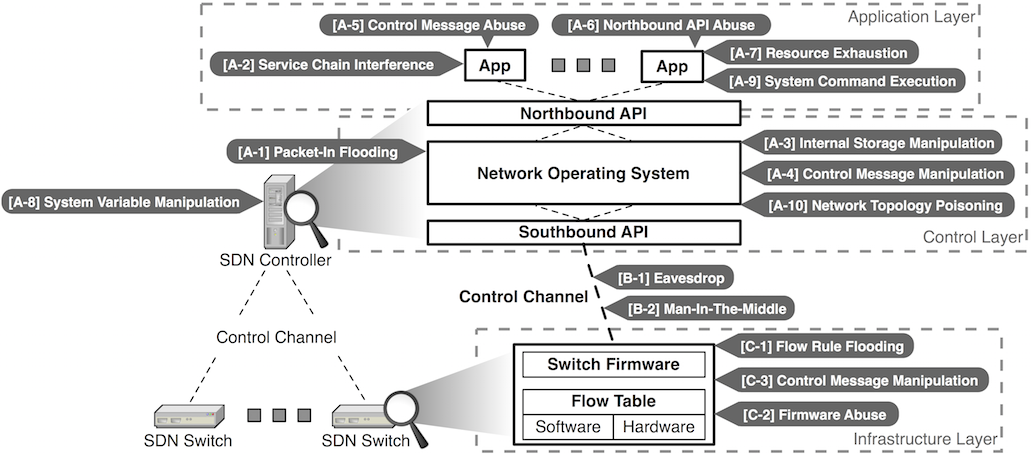
\includegraphics[width=1\textwidth]{threats.png}
  	\caption{Principales menaces sur un réseau SDN}
\end{figure}

	\subsection{Scénarios envisagés}
		Pour éclairer de manière expérimentale le large spectre de menaces auquel peut être soumis un réseau SDN, j'ai mis en place au fur et à mesure 6 preuves de concept, certaines n'étant pas très complexes mais démontrent toutefois certaines faiblesses. Même si parmi les scénarios envisagés il y en a certains qui sont spécifiques à ONOS (notamment ceux qui concernent l'interface nord), on verra que les attaques sont globalement les mêmes que dans un réseau classique, avec en revanche des impacts plus lourds.

Pour rester dans la nomenclature précédente, voici les attaques envisagées :

\begin{itemize}

\item \underline{Scénario 1 :} Tampering et Information disclosure (interface sud) \\
\underline{But :} Intercepter et modifier les communications sur le plan de données ou de contrôle si TLS n'est pas activé.

\item \underline{Scénario 2 :} Spoofing et DoS (interface sud) \\
\underline{But :} Altérer la topologie estimée par le contrôleur en usurpant l'identité d'un switch ou en inventant un faux switch et en créant des faux messages LLDP.

\item \underline{Scénario 3 :} DoS (interface sud) \\
\underline{But :} Réduire fortement le débit au niveau de certains nœuds par envoi d'un très grand nombre de paquets dont on espère qu'ils vont chacun aboutir à la création d'une règle au niveau du contrôleur. Ceci afin de surcharger les tables de flux des switchs visés.

\item \underline{Scénario 4 :} DoS (interface nord) \\
\underline{But :} Altérer les performances du contrôleur, tester certaines permissions critiques avec le Security Mode.

\item \underline{Scénario 5 :} Information disclosure (interface nord) \\
\underline{But :} A partir d'une application banale qui n'a pas le droit de regarder quelles sont les autres applications présentes sur le contrôleur, observer quels éléments peuvent quand même être rendus accessibles sans que cela soit explicitement prévu.

\item \underline{Scénario 6 :} Spoofing (interface nord) \\
\underline{But :} Tester la frontière entre permission liée à une application et permission liée à l'API REST.

\end{itemize}

Chacun de ces 6 scénarios est détaillé séparément dans la partie suivante.
\section{Audit}
	\subsection{Man in the middle au niveau de l'interface sud}
	\subsection{Altération de la topologie depuis l'interface sud}
	\subsection{Deni de service au niveau de l'interface sud}
	\subsection{Deni de service au niveau de l'interface nord}
	\subsection{Fuites d'information au niveau de l'interface nord}
	\subsection{Mauvaise configuration au niveau de l'interface nord}
\section{Validation et évaluation}
	\subsection{Résultats de l'étude}
	\subsection{Autres considérations}
\section{Perspectives à l'issue du stage}
\section{Ressources}


~

\newpage

%récupérer les citation avec "/footnotemark"
\nocite{*}

%choix du style de la biblio
\bibliographystyle{plain}
%inclusion de la biblio
\bibliography{bibliographie.bib}
%voir wiki pour plus d'information sur la syntaxe des entrées d'une bibliographie

\end{document}
